%  LaTeX support: latex@mdpi.com 
%  In case you need support, please attach all files that are necessary for compiling as well as the log file, and specify the details of your LaTeX setup (which operating system and LaTeX version / tools you are using).

%=================================================================
\documentclass[cryptography,article,submit,moreauthors,pdftex]{Definitions/mdpi} 

% If you would like to post an early version of this manuscript as a preprint, you may use preprint as the journal and change 'submit' to 'accept'. The document class line would be, e.g., \documentclass[preprints,article,accept,moreauthors,pdftex]{mdpi}. This is especially recommended for submission to arXiv, where line numbers should be removed before posting. For preprints.org, the editorial staff will make this change immediately prior to posting.

%--------------------
% Class Options:
%--------------------
%----------
% journal
%----------
% Choose between the following MDPI journals:
% acoustics, actuators, addictions, admsci, aerospace, agriculture, agriengineering, agronomy, algorithms, animals, antibiotics, antibodies, antioxidants, applsci, arts, asc, asi, atmosphere, atoms, axioms, batteries, bdcc, behavsci , beverages, bioengineering, biology, biomedicines, biomimetics, biomolecules, biosensors, brainsci , buildings, cancers, carbon , catalysts, cells, ceramics, challenges, chemengineering, chemistry, chemosensors, children, cleantechnol, climate, clockssleep, cmd, coatings, colloids, computation, computers, condensedmatter, cosmetics, cryptography, crystals, dairy, data, dentistry, designs , diagnostics, diseases, diversity, drones, econometrics, economies, education, ejihpe, electrochem, electronics, energies, entropy, environments, epigenomes, est, fermentation, fibers, fire, fishes, fluids, foods, forecasting, forests, fractalfract, futureinternet, futurephys, galaxies, games, gastrointestdisord, gels, genealogy, genes, geohazards, geosciences, geriatrics, hazardousmatters, healthcare, heritage, highthroughput, horticulturae, humanities, hydrology, ijerph, ijfs, ijgi, ijms, ijns, ijtpp, informatics, information, infrastructures, inorganics, insects, instruments, inventions, iot, j, jcdd, jcm, jcp, jcs, jdb, jfb, jfmk, jimaging, jintelligence, jlpea, jmmp, jmse, jnt, jof, joitmc, jpm, jrfm, jsan, land, languages, laws, life, literature, logistics, lubricants, machines, magnetochemistry, make, marinedrugs, materials, mathematics, mca, medicina, medicines, medsci, membranes, metabolites, metals, microarrays, micromachines, microorganisms, minerals, modelling, molbank, molecules, mps, mti, nanomaterials, ncrna, neuroglia, nitrogen, notspecified, nutrients, ohbm, optics, particles, pathogens, pharmaceuticals, pharmaceutics, pharmacy, philosophies, photonics, physics, plants, plasma, polymers, polysaccharides, preprints , proceedings, processes, proteomes, psych, publications, quantumrep, quaternary, qubs, reactions, recycling, religions, remotesensing, reports, resources, risks, robotics, safety, sci, scipharm, sensors, separations, sexes, signals, sinusitis, smartcities, sna, societies, socsci, soilsystems, sports, standards, stats, surfaces, surgeries, sustainability, symmetry, systems, technologies, test, toxics, toxins, tropicalmed, universe, urbansci, vaccines, vehicles, vetsci, vibration, viruses, vision, water, wem, wevj

%---------
% article
%---------
% The default type of manuscript is "article", but can be replaced by: 
% abstract, addendum, article, benchmark, book, bookreview, briefreport, casereport, changes, comment, commentary, communication, conceptpaper, conferenceproceedings, correction, conferencereport, expressionofconcern, extendedabstract, meetingreport, creative, datadescriptor, discussion, editorial, essay, erratum, hypothesis, interestingimages, letter, meetingreport, newbookreceived, obituary, opinion, projectreport, reply, retraction, review, perspective, protocol, shortnote, supfile, technicalnote, viewpoint
% supfile = supplementary materials

%----------
% submit
%----------
% The class option "submit" will be changed to "accept" by the Editorial Office when the paper is accepted. This will only make changes to the frontpage (e.g., the logo of the journal will get visible), the headings, and the copyright information. Also, line numbering will be removed. Journal info and pagination for accepted papers will also be assigned by the Editorial Office.

%------------------
% moreauthors
%------------------
% If there is only one author the class option oneauthor should be used. Otherwise use the class option moreauthors.

%---------
% pdftex
%---------
% The option pdftex is for use with pdfLaTeX. If eps figures are used, remove the option pdftex and use LaTeX and dvi2pdf.

%=================================================================
\firstpage{1} 
\makeatletter 
\setcounter{page}{\@firstpage} 
\makeatother
\pubvolume{xx}
\issuenum{1}
\articlenumber{5}
\pubyear{2020}
\copyrightyear{2020}
%\externaleditor{Academic Editor: name}
\history{Received: date; Accepted: date; Published: date}
%\updates{yes} % If there is an update available, un-comment this line

%% MDPI internal command: uncomment if new journal that already uses continuous page numbers 
%\continuouspages{yes}

%------------------------------------------------------------------
% The following line should be uncommented if the LaTeX file is uploaded to arXiv.org
%\pdfoutput=1

%=================================================================
% Add packages and commands here. The following packages are loaded in our class file: fontenc, calc, indentfirst, fancyhdr, graphicx, lastpage, ifthen, lineno, float, amsmath, setspace, enumitem, mathpazo, booktabs, titlesec, etoolbox, amsthm, hyphenat, natbib, hyperref, footmisc, geometry, caption, url, mdframed, tabto, soul, multirow, microtype, tikz

%=================================================================
%% Please use the following mathematics environments: Theorem, Lemma, Corollary, Proposition, Characterization, Property, Problem, Example, ExamplesandDefinitions, Hypothesis, Remark, Definition, Notation, Assumption
%% For proofs, please use the proof environment (the amsthm package is loaded by the MDPI class).

%=================================================================
% Full title of the paper (Capitalized)
\Title{Dragon Crypto - An innovative cryptosystem}

% Author Orchid ID: enter ID or remove command
\newcommand{\orcidauthorA}{0000-0001-5858-5417} % Add \orcidA{} behind the author's name
\newcommand{\orcidauthorB}{0000-0002-3667-8513} % Add \orcidB{} behind the author's name

% Authors, for the paper (add full first names)
\Author{Awnon Bhowmik $^{1,\dagger,\ddagger}$\orcidA{} and Unnikrishnan Menon $^{1,\ddagger}$\orcidB{}}

% Authors, for metadata in PDF
\AuthorNames{Firstname Lastname, Firstname Lastname and Firstname Lastname}

% Affiliations / Addresses (Add [1] after \address if there is only one affiliation.)
\address{%
$^{1}$ \quad Department of Mathematics and Computer Science, 94-20 Guy R. Brewer Blvd, Jamaica, NY 11451; awnon.bhowmik@yorkmail.cuny.edu\\
$^{2}$ \quad Department of Eletrical and Electronics Engineering, VIT, Vellore Campus, Tiruvalam Rd, Katpadi, Vellore, Tamil Nadu 632014; unnikrishnanr.menon2017@vitstudent.ac.in}

% Contact information of the corresponding author
\corres{Correspondence: awnon.bhowmik@yorkmail.cuny.edu}

% Current address and/or shared authorship
%\firstnote{Current address: Affiliation 3} 
%\secondnote{These authors contributed equally to this work.}
% The commands \thirdnote{} till \eighthnote{} are available for further notes

%\simplesumm{} % Simple summary

%\conference{} % An extended version of a conference paper

% Abstract (Do not insert blank lines, i.e. \\) 
\abstract{In recent years cyber-attacks are continuously developing, therefore security specialists must stay busy in the lab inventing new schemes to keep attackers at bay. In this paper we outline the details of a new crypto system based on the dragon curve fractal. The security level of this scheme is based on multiple private keys, that are crucial for effective encryption and decryption of data. This paper covers how core concepts emerging from fractal geometry can be used as a trapdoor function for a new cryptosystem.}

% Keywords
\keyword{dragon curve; dragon fractal; dragon curve fractal; heighway dragon curve; heighway dragon fractal; cryptography; cryptosystem; crypto system; secure encryption; Iterative Function System; IFS; iteration; precision; trapdoor function}

% The fields PACS, MSC, and JEL may be left empty or commented out if not applicable
%\PACS{J0101}
%\MSC{}
%\JEL{}

%%%%%%%%%%%%%%%%%%%%%%%%%%%%%%%%%%%%%%%%%%
% Only for the journal Diversity
%\LSID{\url{http://}}

%%%%%%%%%%%%%%%%%%%%%%%%%%%%%%%%%%%%%%%%%%
% Only for the journal Applied Sciences:
%\featuredapplication{Authors are encouraged to provide a concise description of the specific application or a potential application of the work. This section is not mandatory.}
%%%%%%%%%%%%%%%%%%%%%%%%%%%%%%%%%%%%%%%%%%

%%%%%%%%%%%%%%%%%%%%%%%%%%%%%%%%%%%%%%%%%%
% Only for the journal Data:
%\dataset{DOI number or link to the deposited data set in cases where the data set is published or set to be published separately. If the data set is submitted and will be published as a supplement to this paper in the journal Data, this field will be filled by the editors of the journal. In this case, please make sure to submit the data set as a supplement when entering your manuscript into our manuscript editorial system.}

%\datasetlicense{license under which the data set is made available (CC0, CC-BY, CC-BY-SA, CC-BY-NC, etc.)}

%%%%%%%%%%%%%%%%%%%%%%%%%%%%%%%%%%%%%%%%%%
% Only for the journal Toxins
%\keycontribution{The breakthroughs or highlights of the manuscript. Authors can write one or two sentences to describe the most important part of the paper.}
\hbadness = 10001
%\setcounter{secnumdepth}{4}
%%%%%%%%%%%%%%%%%%%%%%%%%%%%%%%%%%%%%%%%%%
\begin{document}
%%%%%%%%%%%%%%%%%%%%%%%%%%%%%%%%%%%%%%%%%%

%%%%%%%%%%%%%%%%%%%%%%%%%%%%%%%%%%%%%%%%%%
% \setcounter{section}{-1} %% Remove this when starting to work on the template.
% \section{How to Use this Template}
% The template details the sections that can be used in a manuscript. Note that the order and names of article sections may differ from the requirements of the journal (e.g., the positioning of the Materials and Methods section). Please check the instructions for authors page of the journal to verify the correct order and names. For any questions, please contact the editorial office of the journal or support@mdpi.com. For LaTeX related questions please contact latex@mdpi.com.
% %The order of the section titles is: Introduction, Materials and Methods, Results, Discussion, Conclusions for these journals: aerospace,algorithms,antibodies,antioxidants,atmosphere,axioms,biomedicines,carbon,crystals,designs,diagnostics,environments,fermentation,fluids,forests,fractalfract,informatics,information,inventions,jfmk,jrfm,lubricants,neonatalscreening,neuroglia,particles,pharmaceutics,polymers,processes,technologies,viruses,vision

\section{Introduction}
\begin{flushleft}
    Fractals are just a self replication of a particular pattern. There are many fractals that are found in nature. One such fractal curve is known as \textit{Heighway Dragon}, or simply the \textit{Dragon Curve}. Because this is a fractal, hence it requires an IFS (Iterated Function System). In simple words, we make a simple pattern, put it into a recursive function, before running a loop and calling the function over and over again until our objective is accomplished.
\end{flushleft}

\section{The Dragon Fractal}
\begin{flushleft}
        A fractal is a repetition of an initial geometric shape. This is generated by something known as the Iterative Function System (IFS). The dragon curve is one such fractal. There are multiple ways to generate this fractal. 
\end{flushleft}

\subsection{Generating the Dragon Fractal}
\begin{flushleft}
    This dragon curve fractal, or its generation algorithm forms the basis of this cryptosystem, and hence the proposed name \textit{dragon crypto}. Here, we take an arbitrary string of characters, pass each character through the \textit{Koblitz encoder} to obtain the starting point for the IFS.
\end{flushleft}

\begin{flushleft}
	The iterations of the Dragon curve can easily be generated by folding a strip of paper $n$ number of times. We take a strip of paper and fold it in half to the right.$^{\cite{taming_the_dragon}}$ We fold it in half again, to the right. We continue this process as many times as we want (of course it will be hard to fold after a certain point). Let’s say we do it 2 times.
\end{flushleft}

\begin{flushleft}
    Now we unfold the strip and relax it, and we’ll notice that every bend/corner of the strip has become a $90^{\circ}$ turn. What we have now is the second iteration of the Dragon Curve. If we fold the strip of paper in half for a third time and then open it up, we would get the third iteration and so on…
\end{flushleft}

\begin{center}
    \begin{center}
        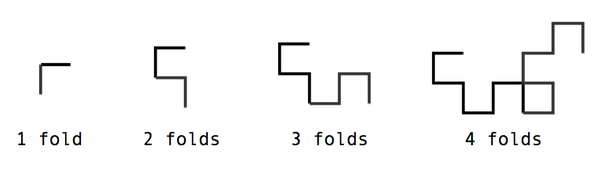
\includegraphics[scale=0.7]{images/paper folding.png}\captionof*{"Paper folding method".png}{Fig 1. \textbf{Paper folding method}}
    \end{center}
\end{center}

\begin{flushleft}
    Now all we have to do is visualize a turtle walking along these lines and it should be able to predict how to move. Let F = forward, L = left, R = right. The following sequences are associated with the respective iterations...
    
    \begin{itemize}
        \item 1st iteration- F L F L
        \item 2nd iteration- F L F L F R F L
        \item 3rd iteration- F L F L F R F L F L F R F R F L
        \vdots
    \end{itemize}

If we know the $n^{\text{th}}$ iteration, we can predict the $(n+1)^{\text{th}}$ iteration in the following way. Let’s say we are trying to derive the third iteration from the second iteration.

    \begin{itemize}
        \item We ignore the last element for now (F L F L F R F). In the remaining elements, if there’s a R, it is replaced by L. And if there is a L, it is replace by a R. The sequence now becomes (F R F R F L F R).
        \item Now, we flip these elements about the mid point. The sequence turns into (R F L F R F R F).
        \item Add the last element which we had ignored in the first step. The sequence becomes (R F L F R F R F L).
        \item Appending the result of step 4 to the 1st iteration and we will have our third iteration ready.
    \end{itemize}

Using this same logic, we can predict the next iterations. A fractal curve generated with $15$ iterations is as follows...

\begin{center}
    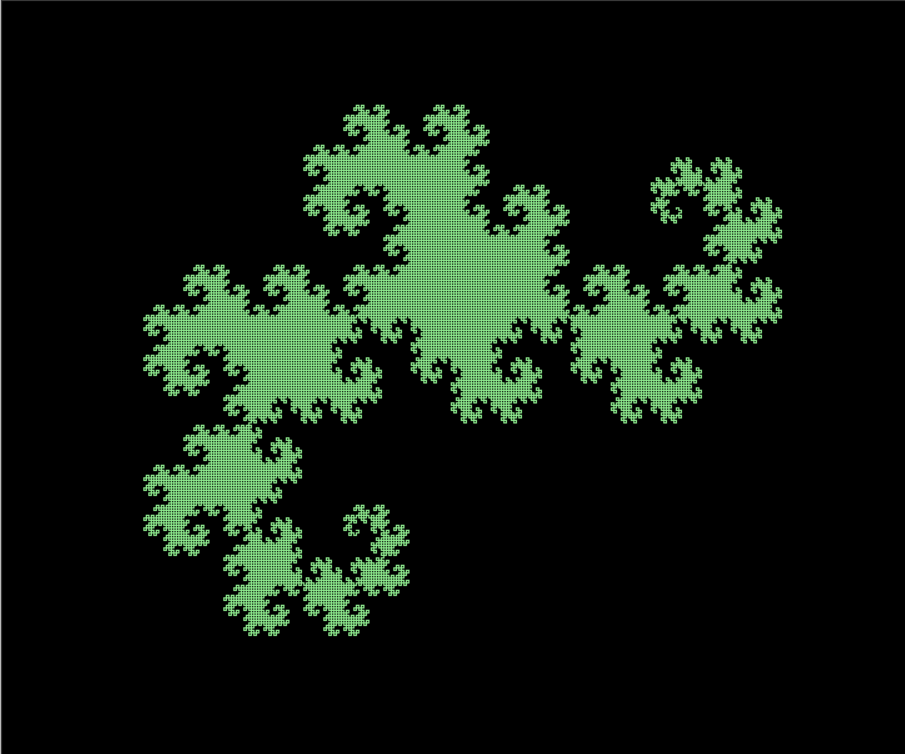
\includegraphics[scale=0.58]{images/dragoncurve.png}\captionof*{"dragoncurve".png}{Fig 2. \textbf{Dragon Curve Fractal}}
\end{center}
\end{flushleft}

\section{Koblitz Encoding \& Decoding Algorithm}
\begin{flushleft}
	The encoding algorithm$^{\cite{koblitz}}$ is as follows...\\
	\begin{itemize}
		\item Given a message $M$, convert each character $m_k$ into a number $a_k$ using Unicode, where $b=2^{16}$ and $0<a_k<2^{16}$
		\item Convert the message $M$ into an integer using $$m=\sum_{k=1}^n a_kb^{k-1}$$. In practice we choose an $n$ to be less than or equal to $160$ such that $m$ satisfies $m\le 2^{16\cdot 160}<p$.
		\item Fix a number $d$ such that $d\le \dfrac{p}{m}$. In practice we choose the prime $p$ large enough so that we can allow $d=100$.
		\item For integers $j=0,1,2,\cdots d-1$  we do the following loop
		\begin{itemize}
			\item Compute the $x$ coordinate of a point on the elliptic curve as $x_j=(dm+j)\mod p$ where $m=\bigg\lfloor{\dfrac{x_j}{d}}\bigg\rfloor$
			\item Compute $s_j=(x_j^3+Ax+B)\mod p$
			\item If $\left(s_j\right)^{\frac{p+1}{2}}\equiv s_j\mod p$, then define $y$ coordinate of a point on the elliptic curve as $y_j=\left(s_j\right)^{\frac{p+1}{4}}\mod p$. Return the point $(x_j,y_j)$.
		\end{itemize}
	\end{itemize}
	
	Thus we are able to encode our message $M$, as an element of the Abelian group $G=E\left(\mathbb{F}_p\right)$.
	
	The decoding algorithm is as follows...\\
	\begin{itemize}
	    \item Consider each point $(x,y)$ and set $m$ to be the greatest integer less than $\dfrac{x-1}k$. Then the point $(x,y)$ decodes as the symbol $m$. 
	\end{itemize}
\end{flushleft}

\section{Trapdoor Function}
\begin{flushleft}
A trapdoor function is a function that is easy to compute in one direction, yet difficult to compute in the opposite direction without special information, called the \textit{trapdoor}. Trapdoor functions came to prominence in cryptography in the mid-1970s with the publication of asymmetric (or public-key) encryption techniques. Several function classes have been proposed, and it soon became obvious that trapdoor functions are harder to find than was initially thought.
\end{flushleft}

\begin{flushleft}
The main novelty of our cryptosystem is the use of \textbf{The Heighway Dragon Fractal} as a trapdoor function. The algorithm starts off with a secret message that needs to be encrypted (called the plainText).
\end{flushleft}

\begin{flushleft}
The Koblitz encoder accepts the plainText along with the curve parameters (obtained from the private key). The koblitz encoder spits out an encoded point in 2D Cartesian space for each character present in the plainText with the help of curve parameters.These points are now the starting point of the dragon curve fractals. For each character, a corresponding starting point and a dragon fractal are generated.
\end{flushleft}

\begin{flushleft}
Now the components of the private key (including size,iterations,angle) are used to generate the the fractal for each character from their corresponding starting points.
\end{flushleft}

\newpage
\begin{flushleft}
\textbf{Private key parameters}
\begin{itemize}
	\item The size defines the length of each forward step.
	\item The Iterations defines the number of iterations for generating the fractal.
	\item The Angle defines the starting angle for the fractal.
	\item Elliptic curve parameters $a$ and $b$ for the function $y^2=x^3+ax+b$
\end{itemize}
\end{flushleft}

\begin{flushleft}
Once the fractals are generated for each encoded starting points, the corresponding ending points are noted and stored.

\begin{align*}
	p_{\text{start}}&=\left\{(x_i,y_i)\right\}\qquad i=1,2,\cdots n\\
	p_{\text{end}}&=\left\{(x_j,y_j)\right\}\qquad j=1,2,\cdots n
\end{align*}
\end{flushleft}

\section{Proposed Algorithm}
    \begin{enumerate}
        \item Input an arbitrary string, and split into list of characters, spaces and special characters
        \item Encryption
        \begin{enumerate}
            \item Pass each character's ASCII representation through the Koblitz encoder (using Koblitz Algorithm in section 3). Every character is then represented by a point $(x_i,y_i)$ on the Cartesian coordinate. Let's call these set of points as initial starting points.
            \item For a fixed length $l$, an angle $\theta$ and a fixed number of iterations $n$ for all characters (or points) in the set, we generate a dragon fractal curve. The end point $(x_j,y_j)$ for each starting point $(x_i,y_i)$ is stored into another list.
            \item A special padding is applied on the list of end points as follows $$"Xx_1Xx_2\cdots Xx_nXYy_1Yy_2\cdots y_nY"$$. This turns it into a string. This string is the encrypted cipher text.
        \end{enumerate}
        
        \item Decryption
        \begin{enumerate}
            \item Remove padding and regenerate points. Parse through each element of the cipher text string and split it at "XY" into $2$ sequences. So now we have $2$ strings:
                \begin{align*}
                    "Xx_1Xx_2\cdots Xx_nX"&\qquad\text{and}\qquad"Yy_1Yy_2\cdots y_nY"
                \end{align*}
            Next, we parse through the $2$ lists and recover the ordered set of end point coordinates $(x_j,y_j)$
            \item The list of end point coordinates are taken and based on the (size, iterations, angle) parameters present in the private key, a dragon curve fractal is generated in reverse by initializing the turtle at an endpoint facing the correct direction based on the angle. If the private key parameters are correct, the reversed dragon fractal will end at the initial starting point. This process is repeated for all characters. The points obtained are stored in a list.
            \item The list of points obtained from the previous step is passed through the \textbf{Koblitz Decoder}. This returns the ASCII values of each character in original string. This is finally converted to string to retrieve original message.
        \end{enumerate}
    \end{enumerate}


\section{Example demonstrating the algorithm}
\begin{center}
    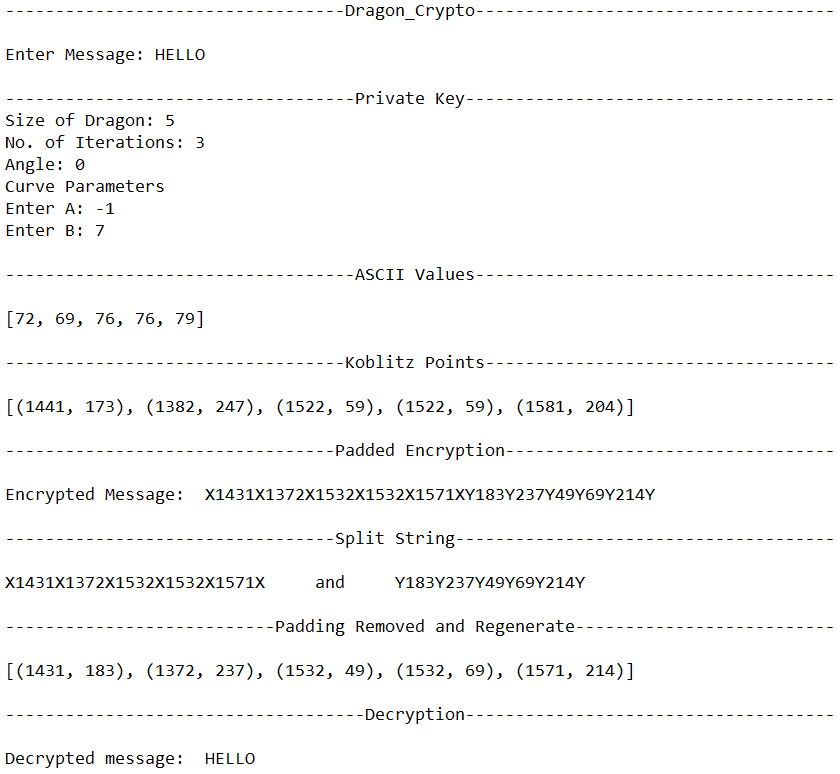
\includegraphics[scale=0.77]{images/output.png}\captionof*{"output".png}{Fig 3. \textbf{Sample Test}}
\end{center}

\section{Conclusions}
\begin{flushleft}
    Cryptography is a 40 year old topic where a lot has been discovered but a lot more yet remains unknown. The essence of any traditional cryptosystem relies on three hard mathematical problems: the integer factorization problem, the discrete logarithm problem or the elliptic curve discrete logarithm problem. Shor's algorithm can be used to easily compromise the security of these conventional cryptosystems. So for a secure future, it is critical to come up with innovative trapdoor functions that can be incorporated in the heart of the encryption scheme.
\end{flushleft}

\begin{flushleft}
   In this paper, we proposed a new encryption algorithm based on the well known dragon curve fractal, due to the fact that not many people have worked on an approach that is closely related to the work discussed here. Whether on not this system is truly usable at the industry level is out of scope of this paper for the moment, but hopefully we will be able to build up on our present research work in the near future. 
\end{flushleft}

\begin{flushleft}
    We have shown that our proposed algorithm is working based on the appropriate parameters. It has been noticed that the run time complexity can be drastically reduced by using smaller number of iterations while increasing the length to compensate for the precision of the endpoint as well as the Euclidean distance from the start point. So far no edge cases have been found, but we suspect the presence of one or more. This is dependent on the calculation precision of the machine. Our work so far is available here.$^{\cite{dragon_crypto}}$
\end{flushleft}

\vspace{6pt} 

%%%%%%%%%%%%%%%%%%%%%%%%%%%%%%%%%%%%%%%%%%
%% optional
%\supplementary{The following are available online at \linksupplementary{s1}, Figure S1: title, Table S1: title, Video S1: title.}

% Only for the journal Methods and Protocols:
% If you wish to submit a video article, please do so with any other supplementary material.
% \supplementary{The following are available at \linksupplementary{s1}, Figure S1: title, Table S1: title, Video S1: title. A supporting video article is available at doi: link.}

%%%%%%%%%%%%%%%%%%%%%%%%%%%%%%%%%%%%%%%%%%
\authorcontributions{Conceptualization, A.B. and U.M.; Methodology, A.B. and U.M.; Software, A.B. and U.M.; Validation, U.M.; Formal analysis, A.B. and U.M.; Writing--original draft preparation, A.B.; Writing--review and editing, A.B.; Visualization, A.B. and U.M. All authors have read and agreed to the submitted version of the manuscript.}

%%%%%%%%%%%%%%%%%%%%%%%%%%%%%%%%%%%%%%%%%%
\funding{The authors received no financial support for this project.}

% %%%%%%%%%%%%%%%%%%%%%%%%%%%%%%%%%%%%%%%%%%
% \acknowledgments{In this section you can acknowledge any support given which is not covered by the author contribution or funding sections. This may include administrative and technical support, or donations in kind (e.g., materials used for experiments).}

%%%%%%%%%%%%%%%%%%%%%%%%%%%%%%%%%%%%%%%%%%
\conflictsofinterest{The authors declare no conflict of interest} 


% Citations and References in Supplementary files are permitted provided that they also appear in the reference list here. 

%=====================================
% References, variant A: internal bibliography
%=====================================
\reftitle{References}
\begin{thebibliography}{999}
% Reference 1
\bibitem[Author1(year)]{koblitz}
Brady, R., Davis, N., \& Tracy, A. (n.d.). Encrypting with Elliptic Curve Cryptography. pp 10. Available Online: \href{https://www.math.purdue.edu/~egoins/notes/Encrypting_Text_Messages_via_Elliptic_Curve_Cryptography.pdf}{\footnotesize{http://www.math.purdue.edu/$\sim$egoins/notes/Encrypting$\_$Text$\_$Messages$\_$via$\_$Elliptic$\_$Curve$\_$Cryptography.pdf}}
% Reference 2
\bibitem[Author2(year)]{dragon_crypto} Bhowmik, A. \& Menon, U.; \textit{Dragon-Crypto}, {\textbf{2020}}. \\Available online: \href{https://github.com/awnonbhowmik/Dragon-Crypto}{https://github.com/awnonbhowmik/Dragon-Crypto}
% Reference 3
\bibitem[Author3(year)]{taming_the_dragon} Bhowmik, A. \& Menon, U.; \textit{Taming The Dragon}, {May \textbf{2018}}. \\Available online: \href{https://www.quora.com/q/rrqrrlbcxwyhoqay/The-Dragon-Curve-Fractal-in-Python}{https://www.quora.com/q/rrqrrlbcxwyhoqay/The-Dragon-Curve-Fractal-in-Python}
\end{thebibliography}

% The following MDPI journals use author-date citation: Arts, Econometrics, Economies, Genealogy, Humanities, IJFS, JRFM, Laws, Religions, Risks, Social Sciences. For those journals, please follow the formatting guidelines on http://www.mdpi.com/authors/references
% To cite two works by the same author: \citeauthor{ref-journal-1a} (\citeyear{ref-journal-1a}, \citeyear{ref-journal-1b}). This produces: Whittaker (1967, 1975)
% To cite two works by the same author with specific pages: \citeauthor{ref-journal-3a} (\citeyear{ref-journal-3a}, p. 328; \citeyear{ref-journal-3b}, p.475). This produces: Wong (1999, p. 328; 2000, p. 475)

%=====================================
% References, variant B: external bibliography
%=====================================
%\externalbibliography{yes}
%\bibliography{your_external_BibTeX_file}

%%%%%%%%%%%%%%%%%%%%%%%%%%%%%%%%%%%%%%%%%%
%% optional
% \sampleavailability{Samples of the compounds ...... are available from the authors.}

%% for journal Sci
%\reviewreports{\\
%Reviewer 1 comments and authors’ response\\
%Reviewer 2 comments and authors’ response\\
%Reviewer 3 comments and authors’ response
%}

%%%%%%%%%%%%%%%%%%%%%%%%%%%%%%%%%%%%%%%%%%
\end{document}

